\setchapterpreamble{\dictum[G. H. Hardy, \textit{A Mathematician's
  Apology}]{``It is a `simple' theorem, simple both in idea and
    execution, but there is no doubt at all about it being a theorem of
    the highest class. It is as fresh and significant as when it was
discovered---two thousand years have not written a wrinkle on it.''}}
\chapter{The Real Numbers}
\begin{theorem}[The irrationality of $\sqrt{2}$]
  There is no rational number whose square is $2$.
\end{theorem}

\begin{proof}
  A rational number is any number that can be expressed in the form
  $p/q$, where $p$ and $q$ are integers. Thus, what the theorem
  asserts is that no matter how $p$ and $q$ are chosen, it is never
  the case that $(p/q)^2 = 2$. The line of attack is indirect, using
  a type of argument referred to as a proof by contradiction. The
  idea is to assume that there is a rational number whose square is 2
  and then proceed along logical lines until we reach a conclusion
  that is unacceptable. At this point, we will be forced to retrace
  our steps and reject the erroneous assumption that some rational
  number squared is equal to 2. In short, we will prove that the
  theorem is true by demonstrating that it cannot be false.

  And so assume, for contradiction, that there exist integers $p$ and
  $q$ satisfying
  \[ \left(\frac{p}{q}\right)^2 = 2. \tag{1} \]
  We may also assume that $p$ and $q$ have no common factor, because,
  if they had one, we could simply cancel it out and rewrite the
  fraction in lowest terms. Now, equation (1) implies
  \[ p^2 = 2q^2. \tag{2} \]
  From this, we can see that the integer $p^2$ is an even number (it
  is divisible by 2), and hence $p$ must be even as well because the
  square of an odd number is odd. This allows us to write $p = 2r$,
  where $r$ is also an integer. If we substitute $2r$ for $p$ in
  equation (2), then a little algebra yields the relationship
  \[ 2r^2 = q^2. \]
  But now the absurdity is at hand. This last equation implies that
  $q^2$ is even, and hence $q$ must also be even. Thus, we have shown
  that $p$ and $q$ are both even (i.e., divisible by 2) when they
  were originally assumed to have no common factor. From this logical
  impasse, we can only conclude that equation (1) cannot hold for any
  integers $p$ and $q$, and thus the theorem is proved.
\end{proof}

\begin{remark}
  So the rationals aren't quite enough. That said, they do have
  almost every other fundamental property we would want. To the
  point: They are what we call an \textit{ordered field}. But first,
  what's a \textit{field}? It's a set that satisfies the classic
  additive and multiplicative properties we know and love.
\end{remark}

\begin{definition}[Fields]
  A \vocab{field} is a nonempty set $\FF$, along with two binary
  operations, addition ($+$) and multiplication ($\cdot$), satisfying
  the following axioms.
  \begin{itemize}
    \item \textbf{Axiom 1 (Commutative Law).} If $a, b \in \FF$, then
      $a + b = b + a$ and $a \cdot b = b \cdot a$.
    \item \textbf{Axiom 2 (Distributive Law).} If $a, b \in \FF$, $a
      \cdot (b + c) = a \cdot b + a \cdot c$.
    \item \textbf{Axiom 3 (Associative Law).} If $a, b \in \FF$, then
      $(a + b) + c = a + (b + c)$ and $(a \cdot b) \cdot c = a \cdot
      (b \cdot c)$.
    \item \textbf{Axiom 4 (Identity Law).} There are special elements
      $\zero, \one \in \FF$, where $a + \zero = a$ and $a \cdot \one
      = a$ for all $a \in \FF$.
    \item \textbf{Axiom 5 (Inverse Law).} For each $a \in \FF$, there
      is an element $-a \in \FF$ such that $a + (-a) = \zero$. If $a
      \neq \zero$, then there is also an element $a^{-\one} \in \FF$
      such that $a \times a^{-\one} = \one$.
  \end{itemize}
\end{definition}

\begin{example}
  Below are some examples and some non-examples of fields.
  \begin{itemize}
    \item The natural number $\NN$ do not form a field; they fail the
      first half of Axiom 4 and both halves of Axiom 5.
    \item The integers $\ZZ$ \textit{almost} form a field; they only
      fail the second half of Axiom 5.
    \item One can check that the rationals $\QQ$ form a field.
  \end{itemize}
\end{example}

\begin{remark}
  Now, let's come up with a definition for an ordered field. Think
  about $\QQ$. What does $\QQ$ have that a field does not? There are
  three main properties we are missing: First, there are infinitely
  many rationals (and they are ``symmetric'' about the 0 element.)
  Second, the rationals have an ordering to them. Lastly, we would
  like to talk about how big a number is. Beautifully,
  \defref{ordered-fields} describes a single elegant axiom that we
  can include to capture \textit{all} of these properties.
\end{remark}

\begin{definition}[Ordered Fields]
  \deflabel{ordered-fields}
  An \vocab{ordered field} is a field $\FF$, along with the following
  additional axiom.

  \textbf{Axiom 6 (Order Axiom).} There is a nonempty subset $P
  \subseteq \FF$, called the \textit{positive elements}, such that
  \begin{enumerate}
    \item If $a, b \in P$, then $a + b \in P$ and $a \cdot b \in P$;
    \item If $a \in \FF$ and $a \neq \zero$, then either $a \in P$ or
      $-a \in P$, but not both.
  \end{enumerate}
\end{definition}

\begin{definition}[Inequalities]
  If $\FF$ is an ordered field and $a, b \in \FF$, then we say that
  ``$a < b$'' if $b - a \in P$. Likewise, $a \leq b$ means that
  either $a = b$ or $a < b$.

  We define ``$>$'' similarly.
\end{definition}

\begin{fact}[Properties of inequalities]
  For $a, b, c$ in an ordered field $\FF$:
  \begin{enumerate}
    \item If $a < b$, then $a + c < b + c$.
    \item Transitivity: If $a < b$ and $b < c$, then $a < c$.
    \item If $a < b$, then $ac < bc$ if $c > 0$, and $ac > bc$ if $c < 0$.
    \item If $a \neq 0$, then $a^2 > 0$.
  \end{enumerate}
\end{fact}

\begin{definition}[The absolute value function]
  If $\FF$ is an ordered field, define the \textit{absolute value}
  function $\abs{\cdot} : \FF \to \FF$ to be
  \begin{align*}
    \abs{x} =
    \begin{cases}
      x, & x \geq 0 \\
      -x, & x < 0.
    \end{cases}
  \end{align*}
\end{definition}

\begin{fact}[Properties of absolute values]
  \faclabel{properties-of-absolute-values}
  For $a, b$ in an ordered field $\FF$:
  \begin{enumerate}
    \item $\abs{a} \geq 0$, with equality if and only if $a = 0$.
    \item $\abs{a} = \abs{-a}$.
    \item $-\abs{a} \leq a \leq \abs{a}$.
    \item $\abs{a \cdot b} = \abs{a} \cdot \abs{b}$.
    \item $1/\abs{a} = \abs{1/a}$, if $a \neq 0$.
    \item $\abs{a/b} = \abs{a}/\abs{b}$, if $b \neq 0$.
    \item $\abs{a} \leq b$ if and only if $-b \leq a \leq b$.
  \end{enumerate}
\end{fact}

\begin{theorem}[The triangle inequality]
  \thmlabel{triangle-inequality}
  If $\FF$ is an ordered field and if $x, y \in \FF$, then
  \[ \abs{x + y} \leq \abs{x} + \abs{y}. \]
\end{theorem}

\begin{proof}
  For $x, y \in \FF$, by \facref{properties-of-absolute-values} part 3 we have
  \[ -\abs{x} \leq x \leq \abs{x} \qquad \text{and} \qquad -\abs{y}
  \leq y \leq \abs{y}. \]
  Adding these two together gives
  \[ -(\abs{x} + \abs{y}) \leq x + y \leq \abs{x} + \abs{y}. \]
  And so, by \facref{properties-of-absolute-values} part 7,
  \[ \abs{x + y} \leq \abs{x} + \abs{y}. \]
\end{proof}

\begin{corollary}[The reverse triangle inequality]
  Assume that $\FF$ is an ordered field and $x, y \in \FF$. Then,
  \begin{align*}
    \abs{\abs{x} - \abs{y}} \leq \abs{x - y}.
  \end{align*}
\end{corollary}

\begin{proof}
  By \facref{properties-of-absolute-values} part 7, it suffices to show that
  \[ -\abs{x - y} \leq \abs{x} - \abs{y} \leq \abs{x - y}. \]
  We first show the right-hand one (that $\abs{x} - \abs{y} \leq
  \abs{x - y}$), and we will do so by applying an application of the
  triangle inequality. Let $a = x - y$ and $b = y$. Then by the
  triangle inequality,
  \[ \abs{a + b} \leq \abs{a} + \abs{b}. \]
  That is,
  \begin{align*}
    \abs{(x - y) + y} \leq \abs{x - y} + \abs{y} \\
    \abs{x} \leq \abs{x - y} + \abs{y}.
  \end{align*}
  Rearranging,
  \[ \abs{x} - \abs{y} \leq \abs{x - y}. \]
  We will use a similar approach to show that $-\abs{x - y} \leq
  \abs{x} - \abs{y}$. Let $c = y - x$ and $d = x$. By the triangle inequality,
  \[ \abs{c + d} \leq \abs{c} + \abs{d} \]
  That is,
  \begin{align*}
    \abs{(y - x) + x} \leq \abs{y - x} + \abs{x} \\
    \abs{y} \leq \abs{y - x} + \abs{x}.
  \end{align*}
  Reaaranging,
  \[ -\abs{y - x} \leq \abs{x} - \abs{y}, \]
  which by \facref{properties-of-absolute-values} part 2 implies that
  \[ -\abs{x - y} \leq \abs{x} - \abs{y}, \]
  as desired.
\end{proof}

\begin{corollary}[Triangle inequality corollaries]
  For both of the following, assume that $\FF$ is an ordered field
  and $x, y \in \FF$.
  \begin{enumerate}
    \item $\abs{x - y} \leq \abs{x} + \abs{y}$.
    \item $\abs{x + y} \geq \abs{\abs{x} - \abs{y}}$.
  \end{enumerate}
\end{corollary}

\begin{proof}
  \phantom{.}

  For part 1, replace $y$ with $-y$ in the triangle inequality.

  For part 2, replace $y$ with $-y$ in the reserve triangle inequality.
\end{proof}

\begin{theorem}[Cauchy-Schwarz inequality]
  If $a_1, \dots, a_n$ and $b_1, \dots, b_n$ are arbitrary real numbers, we have
  \[ \left(\sum_{i = 1}^{n} a_i b_i\right)^2 \leq \left(\sum_{i =
  1}^{n} a_i^2\right) \left(\sum_{i  = 1}^{n} b_i^2\right). \]
\end{theorem}

\begin{proof}
  A sum of squares can never be negative. Hence we have
  \[ \sum_{i = 1}^{n} (a_i x + b_i)^2 \geq 0 \]
  for every $x \in \RR$, with equality if and only if each term is
  zero. This inequality can be written in the form
  \[ Ax^2 + 2Bx + C \geq 0 \]
  where
  \[ A = \sum_{i = 1}^{n} a_i^2, \qquad B = \sum_{i = 1}^n a_i b_i,
  \qquad C = \sum_{i = 1}^{n} b_i^2. \]
  If $A > 0$, put $x = -B/A$ to obtain $B^2 - AC \leq 0$, which is
  the desired inequality. Otherwise if $A = 0$, the rest of the proof
  is trivial.
\end{proof}

\begin{definition}[Upper and lower bounds]
  Let $S$ be an ordered field and $A \subseteq S$ be nonempty.
  \begin{enumerate}
    \item The set $A$ is \textit{bounded above} if there exists some
      $b \in S$ such that $x \leq b$ for all $x \in A$; in this case
      $b$ is called an \vocab{upper bound} of $A$.
    \item The \vocab{least upper bound} of $A$—if it exists—is some
      $b_0 \in S$ such that
      \begin{enumerate}
        \item $b_0$ is an upper bound of $A$, and
        \item if $b$ is any other upper bound of $A$, then $b_0 \leq b$.
      \end{enumerate}
      Such a $b_0$ is also called the \vocab{supremum} of $A$ and is
      denoted $\sup(A)$.
    \item Likewise, the set $A$ is \textit{bounded below} if there
      exists some $b \in S$ such that $x \geq b$ for all $x \in A$;
      in this case, $b$ is called a \vocab{lower bound} of $A$.
    \item Again, like above, the \vocab{greatest lower bound} of
      $A$—if it exists—is some $b_0 \in S$ such that
      \begin{enumerate}
        \item $b_0$ is a lower bound of $A$, and
        \item if $b$ is any other lower bound of $A$, then $b_0 \geq b$.
      \end{enumerate}
      Such a $b_0$ is also called the \vocab{infimum} of $A$ and is
      denoted $\inf(A)$.
    \item If a set is both bounded above and bounded below, then it
      is simply \textit{bounded}.
  \end{enumerate}
\end{definition}

\begin{example}
  The propositions below are left without proof.
  \begin{itemize}
    \item The set $\NN = \set{1, 2, 3, \dots}$ has no upper bounds.
      Lower bounds on $\NN$ include $-17$, $1$, $0.123$, and $-\pi$.
      Note that $\sup(\NN)$ does not exist, but $\inf(\NN)$ = 1.
    \item The set $\QQ$ has no upper or lower bounds; consequently,
      $\sup(\QQ)$ and $\inf(\QQ)$ do not exist.
    \item $\sup(\set{\frac{1}{n} : n \in \NN}) = 1$;
      $\inf(\set{\frac{1}{n} : n \in \NN}) = 0$. Note that the
      supremum here is in the set, while the infimum is not in the set.
    \item $\sup(\set{\frac{n}{n + 1} : n \in \NN}) = 1$;
      $\inf(\set{\frac{n}{n + 1} : n \in \NN}) = \frac{1}{2}$. Note
      that the infimum here is in the set, while the supremum is not in the set.
    \item In $\QQ$ the set $\set{x \in \QQ : x^2 < 2}$ does not have
      a supremum. In $\RR$ it will—in fact, $\sup(\set{x \in \QQ :
      x^2 < 2}) = \sqrt{2}$.
  \end{itemize}
\end{example}

\begin{definition}[Completeness]
  \deflabel{completeness}
  Let $S$ be an ordered field. Then $S$ has the \vocab{least upper
  bound property} if given any nonempty $A \subseteq S$ where $A$ is
  bounded above, $A$ has a least supper bound in $S$. In other words,
  $\sup(A) \in S$ for every such $A$.

  Such a set $S$ is also called \vocab{complete}.
\end{definition}

\begin{theorem}[Existence of $\RR$]
  The real numbers $\RR$ exists, and it is a complete ordered field.
\end{theorem}

\begin{proofsketch}
  We have the ordered field of rational numbers, but they aren't
  complete—there are holes everywhere, and to get to $\RR$ we must
  fill in these gaps. There are several ways to do this. But the most
  common method, which we discuss now, uses \textit{Dedekind cuts}.

  Each real number is going to be a set; at this point we have the
  rationals constructed, so each real number is going to be
  represented by a set of rationals. The way you want to think about
  it is this: the real number $x$ is going to be represented by the
  set of all rational numbers strictly less than $x$. These sets are
  going to be called \textit{cuts}, and while we discuss them you can
  start convincing yourself that each real number will indeed
  correspond to a unique cut, and each cut corresponds to a unique real number.

  \begin{definition}[Dedekind cuts]
    \deflabel{dedekind-cuts}
    A \vocab{cut} should be thought of as the set $(-\infty, b) \cap
    \QQ$. That is, all rational numbers up to a certain point.
    Formally, it is defined as any set $C_b$ satisfying the following
    three conditions.
    \begin{enumerate}
      \item $C_b \subseteq \QQ$, but $C_b \neq \emptyset$ and $C_b \neq \QQ$;
      \item If $p \in C_b$ and $q \notin C_b$, then $p < q$;
      \item If $p \in C_b$, then there exists some $q \in C_b$ where $p < q$.
    \end{enumerate}
  \end{definition}

  And then $\RR$ is defined as the set of all cuts.

  Although we have an intuitive picture of a cut, at the moment it is
  just a set satisfying the above properties. We are interested in
  putting an algebraic structure on this collection of cuts. Addition
  and order work quite smoothly. For a pair of cuts $C_a$ and $C_b$,
  define the following.
  \begin{itemize}
    \item $C_a + C_b := \set{p + q : p \in C_a, q \in C_b}$
    \item $C_a < C_b$ if and only if $C_a \subsetneq C_b$
  \end{itemize}

  One can verify that the addition of two cuts is still a cut, and
  that addition is commutative and associative, that the $\zero$ cut
  behaves as it should (in turn giving \textit{positive} and
  \textit{negative} cuts) and that additive inverses exist. The
  inequality has the property that, given any two cuts $C_a$ and
  $C_b$, exactly one of the following holds: $C_a < C_b$, $C_a =
  C_b$, or $C_b < C_a$.

  Defining multiplication is trickier, because if you simply multiply
  the two sets together you'll have massive negative numbers
  multiplying against each other, creating massive positive numbers.
  Intuitively, you want $C_a \cdot C_b = C_{ab}$. That is, the cut
  $(-\infty, a) \cap \QQ$ times the cut $(-\infty, b) \cap \QQ$
  should equal the cut $(-\infty, a \cdot b) \cap \QQ$; but cuts
  aren't defined with such $a$ and $b$—they produce $a$ and $b$. One
  way around this is to first define multiplication for positive
  cuts. That is, if $C_a$ and $C_b$ are both positive (larger than
  the cut $\set{q \in \QQ : q < 0}$), then define
  \[ C_a \cdot C_b := \set{p \cdot q : p \in C_a, q \in C_b \text{
  with } p, q \geq 0} \cup \set{q \in \QQ : q < 0}. \]
  With this you can then define a product of two negative cuts by
  setting the product equal to the product of the two corresponding
  cuts. To define multiplication between a positive and a negative
  cut, you know the product should be negative so one approach is to
  consider the multiplication when both are positive, and then
  translate the result to the corresponding negative cut. It's a
  hassle to write out, but that's the idea.

  One can then check that the product of two cuts is still a cut,
  that multiplicative inverses exist, and that multiplication is
  commutative and associative, as well as the remaining
  multiplicative/additive distributive and order properties. These
  would be quite annoying to work out in detail, but you can smile
  knowing someone carefully checked them.

  With our set built, and with the algebraic properties defined and
  their properties verified, we now know that $\RR$ is an ordered
  field. All that is left to show is that it is complete. This is
  done by showing that cuts satisfy the \textit{least upper bound
  property}. That is, if $\mathcal{C}$ is a collection of cuts which
  is bounded above (meaning there exists some cut $D$ such that $C
  \leq D$ for all $C \in \mathcal{C}$), then there exists a least
  upper bound (meaning there is a cut $M$ such that $M \leq D$ for
  all upper bounds $D$). The proof is this: Let $M = \bigcup_{C \in
  \mathcal{C}} C$, and show that
  \begin{enumerate}
    \item $M$ is a cut and therefore $M \in \RR$;
    \item $M$ is an upper bound of $\mathcal{C}$, but is smaller than
      all other upper bounds.
  \end{enumerate}
  With those, $\RR$ is a complete ordered field, and hence the real
  numbers are constructed.
\end{proofsketch}

\begin{theorem}[Uniqueness of $\RR$]
  Any complete ordered field is isomorphic to $\RR$.
\end{theorem}

\begin{proofsketch}
  First, let us establish that every complete ordered field $R$ is
  Archimedean. This means that there is no element in $R$ that is
  larger than every finite sum $\one + \one + \dots + \one$. (Why?
    Refer to \lemref{archimedean-principle}. If we let $a = \one$, the
    Archimedean principle states that for any $b$, there exists an $n$
    such that $n \cdot \one > b$. This $n \cdot \one$ is precisely a
  finite sum $\one + \one + \dots + \one$). To prove this property,
  we use contradiction. Suppose there exists such an element, then by
  completeness (\defref{completeness}), there is a least upper bound
  $b$ to these all these finite sums. But then $b - \one$ would also
  be an upper bound, since adding $\one$ to any sum would still be
  less than $b$. This contradicts $b$ being the least upper bound.
  Therefore, no such element exists, and $R$ must be Archimedean.

  Consider two complete ordered fields, $\RR_0$ and $\RR_1$. We
  construct their respective prime subfields, that is, their copies
  of the rationals $\QQ_0$ and $\QQ_1$. This is done by computing
  inside them all the finite quotients of the form $\pm(\one + \one +
  \dots + \one)/(\one + \one + \dots + \one)$, which essentially
  represent all fractions $p/q$ where $p, q \in \ZZ$ and $q > 0$. The
  fractional representation naturally defines an isomorphism between
  $\QQ_0$ and $\QQ_1$. This means that corresponding rational
  elements in each field map to each other, and this mapping
  preserves addition, multiplication, and order. This is illustrated
  in the diagram with the blue dots and arrows connecting
  corresponding rational elements.

  \begin{tightfigure}
    \centering
    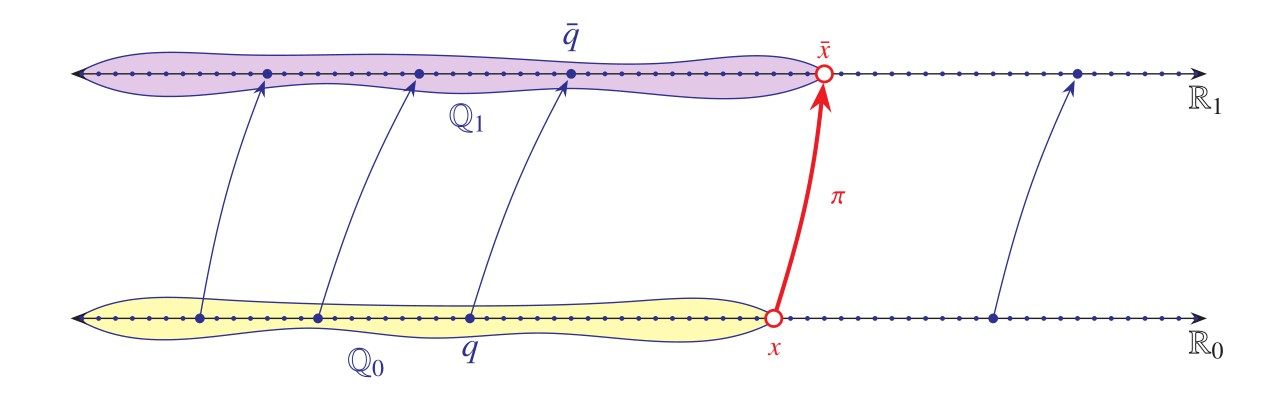
\includegraphics[width=\textwidth]{media/uniqueness-of-the-reals.jpg}
    \vspace{-24pt}
    \caption{An isomorphic mapping $\pi : \RR_0 \to \RR_1$ (courtesy
    of Hamkins \cite{img:uniqueness-of-r}).}
  \end{tightfigure}

  We now extend this isomorphism to the entire fields, $\RR_0$ and
  $\RR_1$, using Dedekind cuts (\defref{dedekind-cuts}). The
  Archimedean property ensures that every element $x$ in $\RR_0$
  defines a unique cut in $\QQ_0$, dividing it into two sets: Those
  rational elements less than $x$ (shown in yellow), and those
  greater than or equal to $x$. Since we have an isomorphism between
  $\QQ_0$ and $\QQ_1$, this cut in $\QQ_0$ corresponds to a similar
  division in $\QQ_1$. By the completeness of $\RR_1$, there must be
  a unique element $\overline{x} \in \RR_1$ that makes this exact
  same cut in $\QQ_1$ (shown in violet). This defines our mapping
  $\pi : x \mapsto \overline{x}$ from $\RR_0$ to $\RR_1$.

  Finally, we verify that the mapping $\pi$ is indeed a field isomorphism:
  \begin{enumerate}
    \item Surjection: Every $y \in \RR_1$ determines a cut in
      $\QQ_1$. By the isomorphism between $\QQ_0$ and $\QQ_1$, this
      corresponds to a cut in $\QQ_0$. By the completeness of
      $\RR_0$, there exists an $x \in \RR_0$ that defines this cut.
      Thus, $\pi(x) = y$.
    \item Injection: If two elements $x_1, x_2 \in \RR_0$ determine
      the same cut in $\QQ_0$, then $x_1 = x_2$ (by the definition of
      Dedekind cuts). Thus, if $\pi(x_1) = \pi(x_2)$, then $x_1$ and
      $x_2$ must define the same cut in $\QQ_0$, which means $x_1 = x_2$.
    \item Field homomorphism: The mapping $\pi$ preserves field
      operations (i.e. addition, multiplication, and order) because
      it is constructed as a continuous extension of the isomorphism
      between the rational subfields $\QQ_0$ and $\QQ_1$.
  \end{enumerate}
  This completes the proof.
\end{proofsketch}

\begin{corollary}[Existence and uniqueness of $\RR$]
  There exists a unique complete ordered field. We call this field
  \textit{the real numbers} $\RR$.
\end{corollary}

\begin{proposition}[Axioms of $\RR$]
  The set $\RR$ has two binary operations, addition ($+$) and
  multiplication ($\cdot$), and is the unique set satisfying the
  following axioms.
  \begin{itemize}
    \item \textbf{Axiom 1 (Commutative Law).} If $a, b \in \RR$, then
      $a + b = b + a$ and $a \cdot b = b \cdot a$.
    \item \textbf{Axiom 2 (Distributive Law).} If $a, b \in \RR$, $a
      \cdot (b + c) = a \cdot b + a \cdot c$.
    \item \textbf{Axiom 3 (Associative Law).} If $a, b \in \RR$, then
      $(a + b) + c = a + (b + c)$ and $(a \cdot b) \cdot c = a \cdot
      (b \cdot c)$.
    \item \textbf{Axiom 4 (Identity Law).} There are special elements
      $\zero, \one \in \RR$, where $a + \zero = a$ and $a \cdot \one
      = a$ for all $a \in \RR$.
    \item \textbf{Axiom 5 (Inverse Law).} For each $a \in \RR$, there
      is an element $-a \in \RR$ such that $a + (-a) = \zero$. If $a
      \neq \zero$, then there is also an element $a^{-\one} \in \RR$
      such that $a \times a^{-\one} = \one$.
    \item \textbf{Axiom 6 (Order Axiom).} There is a nonempty subset
      $P \subseteq \RR$, called the \textit{positive elements}, such that
      \begin{enumerate}
        \item If $a, b \in P$, then $a + b \in P$ and $a \cdot b \in P$;
        \item If $a \in \RR$ and $a \neq \zero$, then either $a \in
          P$ or $-a \in P$, but not both.
      \end{enumerate}
    \item \textbf{Axiom 7 (Completeness Axiom).} Given any nonempty
      $A \subseteq \RR$ where $A$ is bounded above, $A$ has a least
      upper bound. In other words, $\sup(A) \in \RR$ for every such $A$.
  \end{itemize}
\end{proposition}

\begin{proposition}[Suprema are unique]
  If the supremum or infimum of $A \subseteq \RR$ exists, then it is unique.
\end{proposition}

We will only prove that suprema are unique. The infima case is analogous.

\begin{proof}
  Assume for a contradiction that $\alpha$ and $\beta$ are distinct
  least upper bounds of $A$. In particular, both are upper bounds of
  $A$, while $\alpha \neq \beta$. One one hand, since $\alpha$ is a
  least upper bound and $\beta$ is an upper bound, we must have
  $\alpha \leq \beta$. On the other hand, since $\beta$ is a least
  upper bound and $\alpha$ is an upper bound, we must have $\beta
  \leq \alpha$. In summary,
  \[ \alpha \leq \beta \qquad \text{and} \qquad \beta \leq \alpha. \]
  This implies that $\alpha = \beta$, giving our contradiction.
\end{proof}

\begin{theorem}[Square roots exist]
  If $a \in \RR$ and $a \geq 0$, then $\sqrt{a} \in \RR$.
\end{theorem}

\begin{proofidea}
  One can show that $\sqrt{a} = \sup(\set{x \in \RR : x^2 < a})$,
  which is in $\RR$ by completeness.
\end{proofidea}

\begin{theorem}[Suprema analytically]
  \thmlabel{suprema-analytically}
  Let $A \subseteq \RR$. Then $\sup(A) = \alpha$ if and only if
  \begin{enumerate}
    \item $\alpha$ is an upper bound of $A$, and
    \item Given any $\epsilon > 0$, $\alpha - \epsilon$ is
      \textit{not} an upper bound of $A$. That is, there is some $x
      \in A$ for which $x > \alpha - \epsilon$.
  \end{enumerate}
  Likewise, $\inf(A) = \beta$ if and only if
  \begin{enumerate}
    \item $\beta$ is a lower bound of $A$, and
    \item Given any $\epsilon > 0$, $\beta + \epsilon$ is
      \textit{not} a lower bound of $A$. That is, there is some $x
      \in A$ for which $x < \beta + \epsilon$.
  \end{enumerate}
\end{theorem}

We will only prove the suprema case. The infima case is analogous.

\begin{proof}
  \phantom{.}

  $(\Rightarrow)$ First, assume that $\sup(A) = \alpha$. We aim to
  prove part 1 and 2. The first of these is immediate: Since $\sup(A)
  = \alpha$, $\alpha$ is the least upper bound of $A$, which of
  course also implies that it is an upper bound of $A$.

  Now we will show part 2. Let $\epsilon > 0$, Since $\alpha -
  \epsilon < \alpha$, we know that $\alpha - \epsilon$ is not an
  upper bound of $A$, because if so that would contradict $\alpha$
  being the least upper bound of $A$. And so, since $\alpha -
  \epsilon$ is not an upper bound, there must be some $x$ who is
  greater than $\alpha - \epsilon$.

  $(\Leftarrow)$ Now assume part 1 and 2. We aim to prove that
  $\sup(A) = \alpha$. That is, we wish to show that $\alpha$ is an
  upper bound of $A$ (which is implied directly by part 1), and for
  any other upper bound $\beta$, we have $\alpha \leq \beta$. We have
  only the latter to prove. Assume that $\beta$ is some other upper
  bound of $A$, and assume for a contradiction that $\beta < \alpha$.
  Note that $0 < \alpha - \beta$. We will use $(\alpha - \beta)$ as
  our $\epsilon$, and then apply part 2 to contradict $\beta$ being
  an upper bound.

  Now we will work it out formally. Let $\epsilon = \alpha - \beta$.
  Since $\epsilon > 0$, by part 2 there exists some $x \in A$ such
  that $x > \alpha - \epsilon = \alpha - (\alpha - \beta) = \beta$.
  But this is a contradiction, because we assumed that $\beta$ was an
  upper bound of $A$, and yet we found another element $x \in A$ that
  is larger than $\beta$.
\end{proof}

\begin{remark}
  Note that the forward direction of the proof also works well by
  contrapositive. The contrapositive of
  \begin{center}
    $\sup(A) = \alpha$ $\implies$ For all $\epsilon > 0$ there is an
    $x \in A$ such that $x > \alpha - \epsilon$ \\
    \raggedright is \par
    \centering There is an $\epsilon > 0$ such that for all $x \in A$
    we have $x \leq \alpha - \epsilon$ $\implies$ $\sup(A) \neq \alpha$.
  \end{center}
  And to prove this, just observe that the left-hand side implies
  that $\alpha - \epsilon$ is an upper bound of $A$, and so $\sup(A)
  \leq \alpha - \epsilon$, which of course implies that $\sup(A) \neq
  \alpha$, as desired.
\end{remark}

\begin{lemma}[The Archimedean principle]
  \lemlabel{archimedean-principle}
  If $a$ and $b$ are real numbers with $a > 0$, then there exists a
  natural number $n$ such that $na > b$.

  In particular, for any $\epsilon > 0$ there exists $n \in \NN$ such
  that $\frac{1}{n} < \epsilon$.
\end{lemma}

\begin{proof}
  We aim to show that $na > b$ for some $n \in \NN$; by dividing over
  the $a$, we aim to prove that there is some $n \in \NN$ such that
  $n > b/a$. Now, the number $b/a$ is just some real number that we
  know nothing about. In fact, let's just call it $x$. So,
  equivalently, we are trying to prove that given any real number
  $x$, there is some integer $n$ such that $n > x$.

  Assume for a contradiction that there is no integer larger than
  $x$. That is, assume that $x$ is an upper bound on the set $\NN$.
  Then $\NN$ is a subset of $\RR$ that is bounded above, and so by
  the completeness of $\RR$ we deduce that $\sup(\NN)$ exists. Call
  this supremum $\alpha$. Since $\alpha$ is the least upper bound of
  $\NN$, we know that $\alpha - 1$ is not an upper bound. That is,
  there exists some integer $m > \alpha - 1$. Adding 1 to each side,
  \[ m + 1 > \alpha. \]
  But this is a contradiction. If $\alpha$ is the supremum of $\NN$,
  then it is an upper bound on $\NN$. But we found $(m + 1) \in \NN$
  which is larger than $\alpha$. This concludes the first statement
  in the principle.

  The second part follows directly from the first by letting $a =
  \epsilon$ and $b = 1$, and dividing over the $n$.
\end{proof}

\begin{example}
  Show that $\inf(\set{\frac{1}{n} : n \in \NN}) = 0$.
  \begin{proof}
    Let $A = \set{\frac{1}{n} : n \in \NN}$. We will use the analytic
    definition of suprema (\thmref{suprema-analytically}). We must
    then show that 0 is a lower bound of $A$ and that, for all
    $\epsilon > 0$, $0 + \epsilon$ is not a lower bound of $A$.

    The first of these is almost immediate: Since 1 and $n$ are
    positive for each $n \in \NN$, so is $1/n$. So $1/n > 0$, and
    thus 0 is indeed a lower bound for $A$.

    Working toward the second, let $\epsilon > 0$. Then by the
    Archimedean principle (\lemref{archimedean-principle}), there
    exists some $n \in \NN$ such that $\frac{1}{n} < \epsilon$. This
    element, $\frac{1}{n}$, is in $A$ and is less than $0 +
    \epsilon$. So $0 + \epsilon$ is not a lower bound of $A$.
  \end{proof}
\end{example}

\begin{example}
  Show that $\sup(\set{\frac{1}{n} : n \in \NN}) = 1$.
  \begin{proof}
    Let $A = \set{\frac{1}{n} : n \in \NN}$. We will use the analytic
    definition of suprema (\thmref{suprema-analytically}). We must
    then show that 1 is an upper bound of $A$ and that, for all
    $\epsilon > 0$, $1 - \epsilon$ is not an upper bound of $A$.

    For the first of these, note that since $n \geq 1$ for all $n \in
    \NN$, and by dividing over the $n$ we have that $1 \geq
    \frac{1}{n}$ for all $n \in \NN$. So 1 is indeed an upper bound for $A$.

    Working towards the second, let $\epsilon > 0$. We need to show
    that there is some $x \in A$ such that $1 - \epsilon < x$. But
    this is always accomplished by the number 1: Clearly $1 \in A$
    and $1 - \epsilon < 1$.
  \end{proof}
\end{example}

\begin{theorem}[$0.999\ldots = 1$]
  \thmlabel{0.999...=1}
  $0.999\dots$ is a repeating decimal representation of the real number 1.
\end{theorem}

\begin{proofidea}
  If we place $0.9, 0.99, 0.999, \dots$ on the real number line, we
  see immediately that all these points are to the left of 1, and
  that they get closer and closer to 1. For any number $x$ that is
  less than 1, the sequence $0.9, 0.99, 0.999, \dots$ will eventually
  reach a number larger than $x$. So it does not make sense to
  identify $0.999\ldots$ with any number less than 1. This means that
  $0.999\ldots$ must be equal to 1.
\end{proofidea}

\begin{proof}
  Let $0.(9)_n$ denote the number $0.999\ldots9$ with $n$ nines after
  the decimal point. For example, $0.(9)_1 = 0.9$, $0.(9)_2 = 0.99$,
  $0.(9)_3 = 0.999$, and so on. Observe that for each $n \in \NN$, we have
  \[ 1 - 0.(9)_n = \frac{1}{10^n}. \]

  Now, let $x = 0.999\ldots$. Clearly, $0.(9)_n < x \leq 1$ for every
  $n \in \NN$. Subtracting these inequalities from 1 gives us
  \[ 0 \leq 1 - x < 1 - 0.(9)_n = \frac{1}{10^n}. \]
  By the Archimedean principle (\lemref{archimedean-principle}),
  there is no positive number smaller than
  \[ \qquad \qquad \frac{1}{10^n} \quad \text{for all $n \in \NN$}. \]
  Therefore, $1 - x$ must be equal to 0. That is, $x = 1$.
\end{proof}

\begin{remark}
  Despite the persistent rumors, $0.999\ldots$ is not
  ``almost exactly 1'' or ``very, very nearly but not quite 1'' or
  ``1's clingy little sibling.'' Rather, $0.999\ldots$ and 1 are, in
  fact, the same number. So the next time someone insists otherwise,
  feel free to hand them a copy of these notes.
\end{remark}

\begin{remark}
  The Archimedean principle used in \thmref{0.999...=1} differs from
  the one stated in \lemref{archimedean-principle}. One can show that
  these two formulations are equivalent.
\end{remark}

\begin{remark}
  We will revisit \thmref{0.999...=1} in future chapters and discuss
  various different proofs.
\end{remark}

\begin{definition}[Density]
  Suppose $A$ and $B$ are ordered field. Then $A$ is \vocab{dense} in
  $B$ if, for any $x, y \in B$, there exists $a \in A$ such that $x < a < y$.
\end{definition}

\begin{example}
  The propositions below are left without proof.
  \begin{itemize}
    \item $\QQ$ is dense in $\QQ$.
    \item $\RR \setminus \QQ$ is dense in $\QQ$.
    \item $\ZZ$ is \textit{not} dense in $\QQ$.
  \end{itemize}
\end{example}

\begin{lemma}
  \lemlabel{precursor-to-q-is-dense-in-r}
  Let $x, y \in \RR$. If $y - x > 1$, then there exists $z \in \ZZ$
  such that $x < z < y$.
\end{lemma}

\begin{proof}
  First assume that $x$ and $y$ are at least 0, and consider the set
  \[ A = \set{n \in \NN_0 : n \leq x}. \]
  Since $x \geq 0$, this set is non-empty, and since it is a set of
  nonnegative integers which is bounded above by $x$, this set is
  finite. By induction on the size of $A$, we can show that $\max(A)$
  exists and is an element of $A$. Call this maximum $M$. We claim $z
  := M + 1$ works.

  Note that since $M \in \NN_0$, also $z \in \NN_0$. Furthermore,
  since $z$ is larger than the largest element of $A$, $z$ is not in
  $A$, implying that $x < z$. Finally,
  \[ M \leq x \qquad \text{implies that} \qquad M + 1 \leq x + 1 \leq y. \]
  So $z < y$. In summary, we have shown that $x < z < y$, as desired.

  The cases where $x$ and $y$ are not at least 0 are similar. If both
  are negative, then by considering $-x$ and $-y$ the above argument
  gives an integer $z$ where $-y < z < -x$, showing that $-z$ works,
  since $x < -z < y$. If one is positive and one is negative, then 0 works.
\end{proof}

\begin{theorem}[$\QQ$ is dense in $\RR$]
  \thmlabel{q-is-dense-in-r}
  The rational numbers are dense in the real numbers.
\end{theorem}

\begin{proof}
  Pick any $x, y \in \RR$ where $x < y$. We need to show that there
  exists some $\frac{m}{n} \in \QQ$ (with $m, n \in \ZZ$) such that
  \[ x < \frac{m}{n} < y. \]
  First note that if $x < 0 < y$ then we are done, since $0 \in \QQ$.
  Furthermore, if we can show that the theorem holds for the case
  that $x$ and $y$ are positive, then it holds when they are negative
  ($0 < x < \frac{m}{n} < y$ implies $-y < \frac{-m}{n} < -x < 0$),
  so we may assume $x$ and $y$ are positive.

  Since $y - x > 0$, by the Archimedean principle
  (\lemref{archimedean-principle}) there exists some $n \in \NN$ such
  that $n (y - x) > 1$; i.e. $ny - nx > 1$. And so, by
  \lemref{precursor-to-q-is-dense-in-r}, there is some integer $m$ with
  \[ nx < m < ny. \]
  That is,
  \[ x < \frac{m}{n} < y, \]
  which concludes the proof.
\end{proof}

\begin{remark}
  The proof of \lemref{precursor-to-q-is-dense-in-r} also implies
  that, for any $x \in \RR$, there exists an integer $M$ such that $M
  \leq x \leq M + 1$. In particular, it implies that the floor and
  ceiling functions exist.
\end{remark}

\begin{definition}[Floor and ceiling functions]
  Let $x \in R$.
  \begin{itemize}
    \item The \textit{floor} of $x$, denoted $\floor{x}$, is the
      integer $n$ such that $x  - 1 < n \leq x$.
    \item The \textit{ceiling} of $x$, denoted $\ceil{x}$, is the
      integer $n$ such that $x \leq n < x + 1$.
  \end{itemize}
\end{definition}

\begin{definition}[Closed and open intervals]
  Define the \textit{closed interval} $[a, b]$ to be $\set{x \in \RR
  : a \leq x \leq b}$. Likewise the \textit{open interval} $(a, b)$
  is defined to be $\set{x \in \RR : a < x < b}$, and half-open
  intervals and intervals to $\pm\infty$ are again exactly as you would expect.
\end{definition}

\begin{theorem}[Characterization of intervals]
  Let $S$ be a subset of $\RR$ that contains at least two points. If
  $S$ has the property such that
  \[ \text{if $x, y \in S$ and $x < y$, then $[x, y] \subseteq S$}, \tag{1} \]
  then $S$ is an interval.
\end{theorem}

\begin{proof}
  There are four cases to consider: (1) $S$ is bounded, (2) $S$ is
  bounded above but not below, (3) $S$ is bounded below but not
  above, and (4) $S$ is neither bounded above nor below.

  \textbf{Case (1).} Let $a = \inf(S)$ and $b = \sup(S)$. Then $S
  \subseteq [a, b]$ and we will show that $(a, b) \subseteq S$. If $a
  < z < b$, then $z$ is not a lower bound of $S$, so there exists $x
  \in S$ with $x < z$. Also, $z$ is not an upper bound of $S$, so
  there exists $y \in S$ with $z < y$. Therefore, $z \in [x, y]$, so
  property (1) implies that $z \in S$. Since $z$ is an arbitrary
  element of $(a, b)$, we conclude that $(a, b) \subseteq S$. Now if
  $a \in S$ and $b \in S$, then $S = [a, b]$. If $a \notin S$ and $b
  \notin S$, then $S = (a, b)$. The other possibilities lead to
  either $S = (a, b]$ or $S = [a, b)$.

  \textbf{Case (2).} Let $b = \sup(S)$. Then $S \subseteq (-\infty,
  b]$ and we will show that $(-\infty, b) \subseteq S$. If $z < b$,
  then $z$ is not an upper bound of $S$, so there exists $y \in S$
  with $z < y$. Also, since $S$ is not bounded below, there exists $x
  \in S$ with $x < z$. By property 1, $z \in [x, y] \subseteq S$.
  Since $z$ is an arbitrary element of $(-\infty, b)$, we conclude
  that $(-\infty, b) \subseteq S$. Now if $b \in S$, then $S =
  (-\infty, b]$, and if $b \notin S$, then $S = (-\infty, b)$.

  \textbf{Case (3).} Let $a = \inf(S)$. Then $S \subseteq [a,
  \infty)$ and we will show that $(a, \infty) \subseteq S$. If $a <
  z$, then $z$ is not a lower bound of $S$, so there exists $x \in S$
  with $x < z$. Also, since $S$ is not bounded above, there exists $y
  \in S$ with $z < y$. By property 1, $z \in [x, y] \subseteq S$.
  Since $z$ is an arbitrary element of $(a, \infty)$, we conclude
  that $(a, \infty) \subseteq S$. Now if $a \in S$, then $S = [a,
  \infty]$, and if $a \notin S$, then $S = (a, \infty)$.

  \textbf{Case (4).} We will show that $S = (-\infty, \infty)$. Pick
  any $x, y \in S$ with $x < y$, property 1 implies that $[x, y]
  \subseteq S$. Since $S$ is neither bounded above nor below, and the
  choice of $x$, $y$ is arbitrary, we conclude that $(-\infty,
  \infty) \subseteq S$. Also, every subset of $\RR$ is a subset of
  $(-\infty, \infty)$, thus $S = (-\infty, \infty)$.
\end{proof}

\begin{theorem}[The nested intervals property]
  \thmlabel{nested-intervals-property}
  For each $n \in \NN$, assume we are given a closed interval $I_n =
  [a_n, b_n]$. Also, assume that each $I_n$ contains $I_{n + 1}$.
  Then, the resulting nested sequence of closed intervals
  \begin{align*}
    I_1 \supseteq I_2 \supseteq I_3 \supseteq I_4 \supseteq \dots
  \end{align*}
  has a nonempty intersection. That is,
  \begin{align*}
    \bigcap_{n = 1}^{\infty} I_n \neq \emptyset.
  \end{align*}
\end{theorem}

\begin{proof}
  In order to show that $\bigcap_{n = 1}^{\infty} I_n \neq \emptyset$
  is not empty, we are going to use the completeness axiom to produce
  a single real number $x$ satisfying $x \in I_n$ for every $n \in
  \NN$. Now, the completeness axiom is a statement about bounded
  sets, and the one we want to consider is the set
  \[ A = \set{a_n : n \in \NN} \]
  of left-hand endpoints of the interval. Because the intervals are
  nested, we see that every $b_n$ serves as an upper bound for $A$.
  Thus, we are justified in setting
  \[ x = \sup(A). \]
  Now, consider a particular $I_n = [a_n, b_b]$. Because $x$ is an
  upper bound for $A$, we have $a_n \leq x$. The fact that each $b_n$
  is an upper bound for $A$ and that $x$ is the least upper bound
  implies $x \leq b_n$.

  Altogether then, we have $a_n \leq x \leq b_n$, which means $x \in
  I_n$ for every choice of $n \in \NN$. Hence, $x \in \bigcap_{n =
  1}^{\infty} I_n$, and the intersection is not empty.
\end{proof}

\begin{remark}
  Note that the conclusion of \thmref{nested-intervals-property} need
  not hold if each $I_n$ is allowed to be an open interval.
\end{remark}
